\documentclass[12pt]{article}

\usepackage[utf8]{inputenc}
\usepackage[english]{babel}
\usepackage{natbib}
\usepackage[T1]{fontenc}
\usepackage{setspace}
\usepackage{graphicx}
\usepackage{hyperref}


\graphicspath{ {images/} }

\title{\vspace{2cm}\textbf{Enterprise Programming}\\6G6Z1103}
\author{Joshua Michael Ephraim Bridge\\14032908\\joshua.m.bridge@stu.mmu.ac.uk}

\pagestyle{headings}

\begin{document}

\maketitle

\tableofcontents

\newpage

\section{Design Patterns}
  \subsection{Model-view-controller}
  \subsection{Static Factory}

\section{Libraries (\& Tools)}
  In this section I will talk a little about each of the main third-party libraries I used, why I chose to use them, and how it helped me solve a problem I was facing - or how it reduced reliance on custom code.

  \subsection{Maven}
    While Maven (\url{http://maven.apache.org}) is not technically a library (more a build automation/project management tool), it does come under the umbrella of tools which helped implement a solution. Another well-known tool like this is Gradle (\url{https://gradle.org}), however this is often used for more complex build management which wasn't really what I needed. I only really needed dependency management within this project as there were a lot of dependencies, and Maven is a lot simpler to set up for this task. Without dependency management I would've had to download individual ‘.jar’ files for each library (which each have their own dependencies to download) and manage them across different computers when developing or testing on other machines. It is also a lot easier to change the version of a dependency if there are compatibility issues between different libraries which rely on each other. Finally as my project was developed in git (\url{https://git-scm.com}), dependency management meant I did not have to host large jar files in the repository.

  \subsection{Spring MVC}
    When developing pretty much any Java application, Spring (\url{https://projects.spring.io/spring-framework/}) is an obvious and hugely popular choice for making developing a lot simpler and more focused on business logic than things like dependency injection. Spring MVC is a part of the framework which focuses on web serving applications traditionally using the MVC structure. Spring MVC allows a REST \citep{fielding2000architectural} service to be easily configured,
    % TODO finish this

    \begin{figure}[ht]
      \centering
      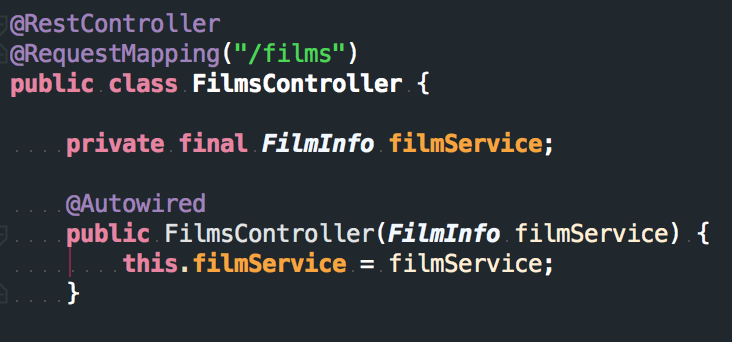
\includegraphics[width=9cm]{autowired-components}
      \caption{Spring's automatic dependency injection}
      \label{fig:spring-autowired-components}
    \end{figure}

  \subsection{Spring HATEOAS}
    Spring HATEOAS (\url{http://projects.spring.io/spring-hateoas/}) is a library that extends a lot of Spring MVC functionality to provide REST representations of objects - by following the HATEOAS principles underlined by \cite{fielding2000architectural}. This framework allowed me to easily map a resource to its URI and include that in the response body. While I feel that this library is quite cumbersome just for adding a URI to an object, the alternative seemed to require assuming the URI would never change (or require changing it in multiple places if it did). The last alternative was to manually \& dynamically find out the servlet URI's, however this seemed needless when Spring HATEOAS does this by design.

  \subsection{Objectify}
    Objectify (\url{https://github.com/objectify/objectify}) is a JPA-like library which allows you to easily connect to Google datastore, and is the library reccomended by Google for doing so in a Java program. Previously I had built the DAO using Hibernate (\url{http://hibernate.org}), however this was not compatibile with Google datastore due to non-compliance with Google's proprietary GQL language. While this worked well for what it was required to do, I ended up having to sacrifice some design points that Hibernate had previously allowed me to use. For example, with Hibernate you are able to declare class fields as ‘final’ - with objectify this is not possible as it sets the values after object initialisation.

  \subsection{Guava}
    Google Guava (\url{https://github.com/google/guava}) is a very useful set of libraries that introduce a lot of new functionality to Java. While I originally made more use of this library when I first started the application and have since refactored most uses out of the code, it is still used for array/map initialisation with a static factory, to hide the ugliness of object initialisation that can often be distracting.

  \subsection{Apache Commons Text}
    Apache Commons Text (\url{https://commons.apache.org/proper/commons-text/}) is a set of useful utility libraries dealing with Strings/text. I used this library for its ToStringBuilder class, which uses reflection to create a string representation of a java object - eliminating the need for custom ‘toString’ methods for every data object.

  \subsection{Gson}
    Google Gson (\url{https://github.com/google/gson}) is a library for automatic serialization from a java object to a JSON string. While Jackson Databind (section \ref{jackson-databind}) is able to handle JSON serialization, I decided to use Gson for this task as Spring MVC has some utilities for integrating with Gson. However I feel as though a relatively similar result could have been achieved using Jackson Databind for both XML and JSON serialization.

  \subsection{Jackson Databind}
    \label{jackson-databind}
    Jackson Databind (\url{https://github.com/FasterXML/jackson-databind}) is a library for object serialization, which has several extensions to allow it to convert objects into many different formats such as JSON and XML. Databind is also highly integrated into Spring MVC, so much so that even just having the library in the classpath allows spring to automatically start serializing, without any code needed. This is also possible with JAXB.
    % TODO jaxb??

  \subsection{JQuery}
    JQuery (\url{http://jquery.com}) is a front-end JavaScript library which simplifies a wide range of tasks that would be a lot more difficult if written in plain JavaScript. It was very useful for removing a lot of procedural code for doing ajax calls to my web services, from retrieving the data to displaying it on the page. I also used JQuery for handling UI elements such as displaying forms, and laying out object data into an HTML table. I did consider using JQuery UI (\url{http://jqueryui.com}) however I found it did not offer any UI elements I felt the need to use, so it would have been needless baggage if I had tried to incorporate it into the front-end.

\section{Refactoring}

\bibliographystyle{agsm}
\bibliography{report}

\end{document}
